\documentclass[10pt,a4paper]{article}
\usepackage[utf8]{inputenc}
\usepackage[T1]{fontenc,url}
\usepackage{multicol}
\usepackage{multirow}
\usepackage{parskip}
\usepackage{lmodern}
\usepackage{microtype}
\usepackage{verbatim}
\usepackage{amsmath, amssymb}
\usepackage{tikz}
\usepackage{physics}
\usepackage{mathtools}
\usepackage{algorithm}
\usepackage{algpseudocode}
\usepackage{listings}
\usepackage{enumerate}
\usepackage{enumitem}
\usepackage{graphicx}
\usepackage{float}
\usepackage{hyperref}
\usepackage{tabularx}
\usepackage{siunitx}
\usepackage{fancyvrb}
\usepackage{xcolor}
\usepackage[margin=3cm]{geometry}
\renewcommand{\baselinestretch}{1}
\renewcommand{\b}{\textbf}
\renewcommand{\exp}{e^}


\begin{document}

\section*{Ordinary Differential Equations}

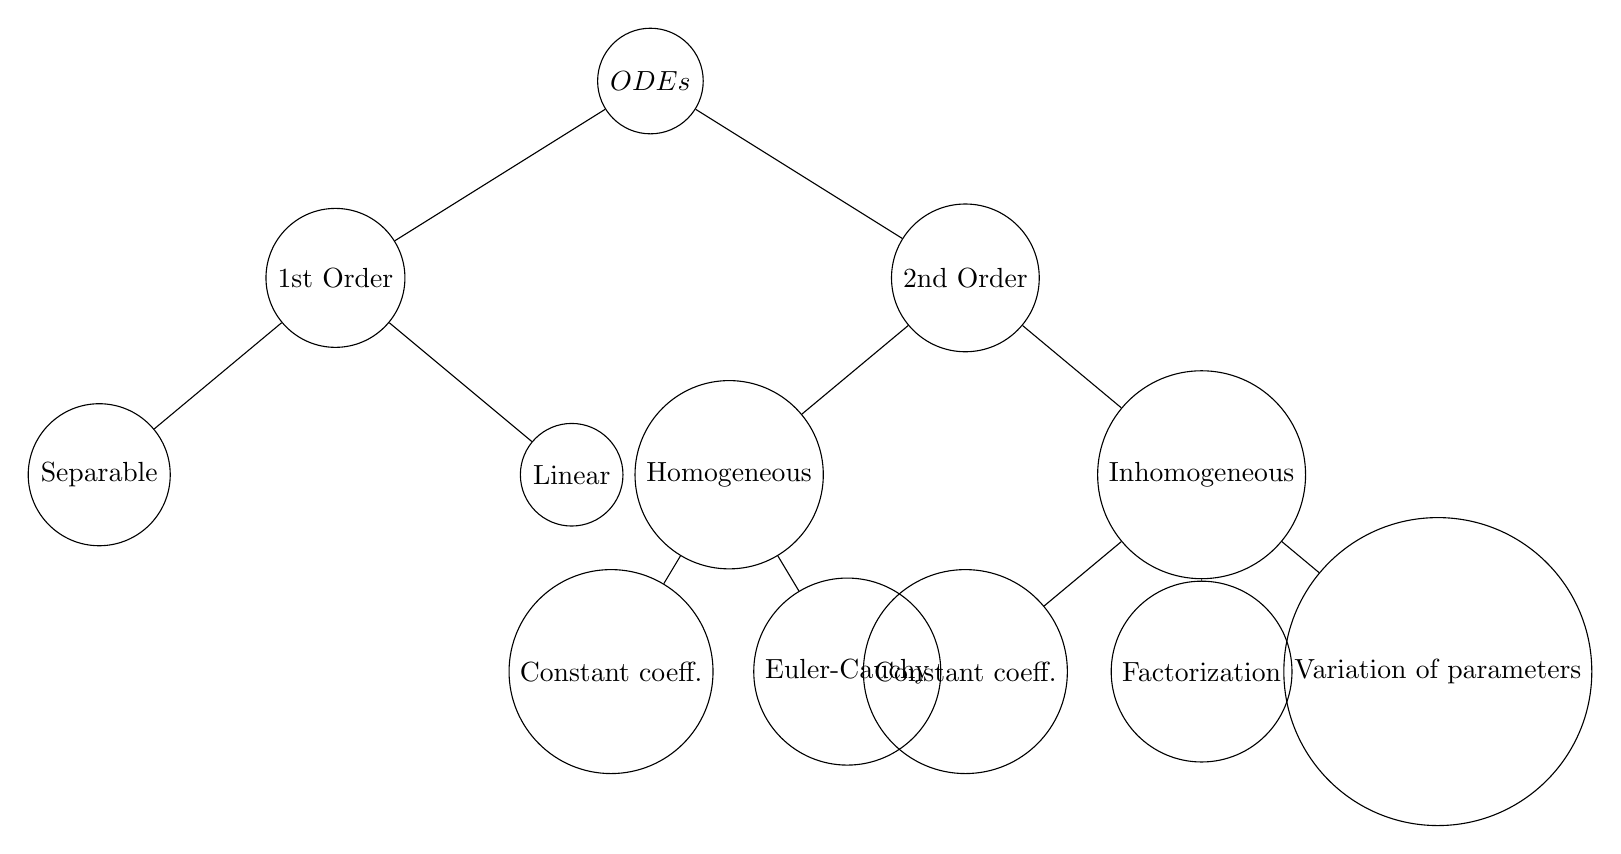
\begin{tikzpicture}[level distance=2.5cm,
  level 1/.style={sibling distance=8cm},
  level 2/.style={sibling distance=6cm},
  level 3/.style={sibling distance=3cm}]
    \node[circle, draw](z){$ODEs$}
        child{node[circle,draw]{1st Order}
            child{node[circle,draw]{Separable}}
            child{node[circle,draw]{Linear}}
            }
        child{node[circle,draw]{2nd Order}
            child{node[circle,draw]{Homogeneous}
                child{node[circle,draw]{Constant coeff.}}
                child{node[circle,draw]{Euler-Cauchy}}
                }
            child{node[circle,draw]{Inhomogeneous}
                child{node[circle,draw]{Constant coeff.}}
                child{node[circle,draw]{Factorization}}
                child{node[circle,draw]{Variation of parameters}}
                }
            };
\end{tikzpicture}

\subsection*{First Order, Linear, ODEs - Integrating Factor}
\[
    y'(x) + P(x) y(x) = Q(x)
\]

\[
    y(x)\mu(x) = \int Q(x)\mu(x) \dd{x} + C \quad\quad\text{with}\quad\quad \mu(x) = \exp{\int P(x)\dd{x}}
\]


\[
    \int (uv') = uv - \int(u'v)
\]



\subsection*{Second Order, Homogenous, Linear ODEs, with constant coefficients - Particular Equation}
\[
    y''(x) + ay'(x) + by(x) = 0
\]

Solve the particular equation
\[
    \lambda^2 + a\lambda + b = 0
\]
for $\lambda_1$ and $\lambda_2$.


\subsubsection*{Two, real roots}
\[
    y(x) = C_1\exp{\lambda_1 x} + C_2\exp{\lambda_2 x}
\]


\subsubsection*{One, real root}
\[
    y(x) = (C_1 + xC_2)\exp{\lambda x}
\]


\subsubsection*{Two, complex roots}
\[
    y(x) = A\exp{\lambda_1 x} + B\exp{\lambda_2 x} = \exp{-a/2 x}\qty[A\exp{i\omega x} + B\exp{-i\omega x}] = \exp{-a/2 x}\qty[\hat{A}\cos{\omega x} + \hat{B}\sin{\omega x}]
\]



\end{document}
